\subsection{Implementation}
Push notifications are centralized on Google and Apple servers for security reasons. For this reason, our application makes use of the \textbf{Firebase cloud messaging} service. This allows us to avoid implementing communication towards APNs which is all handled by Firebase making the notification service almost completely transparent to the developer.

\hspace*{-1cm}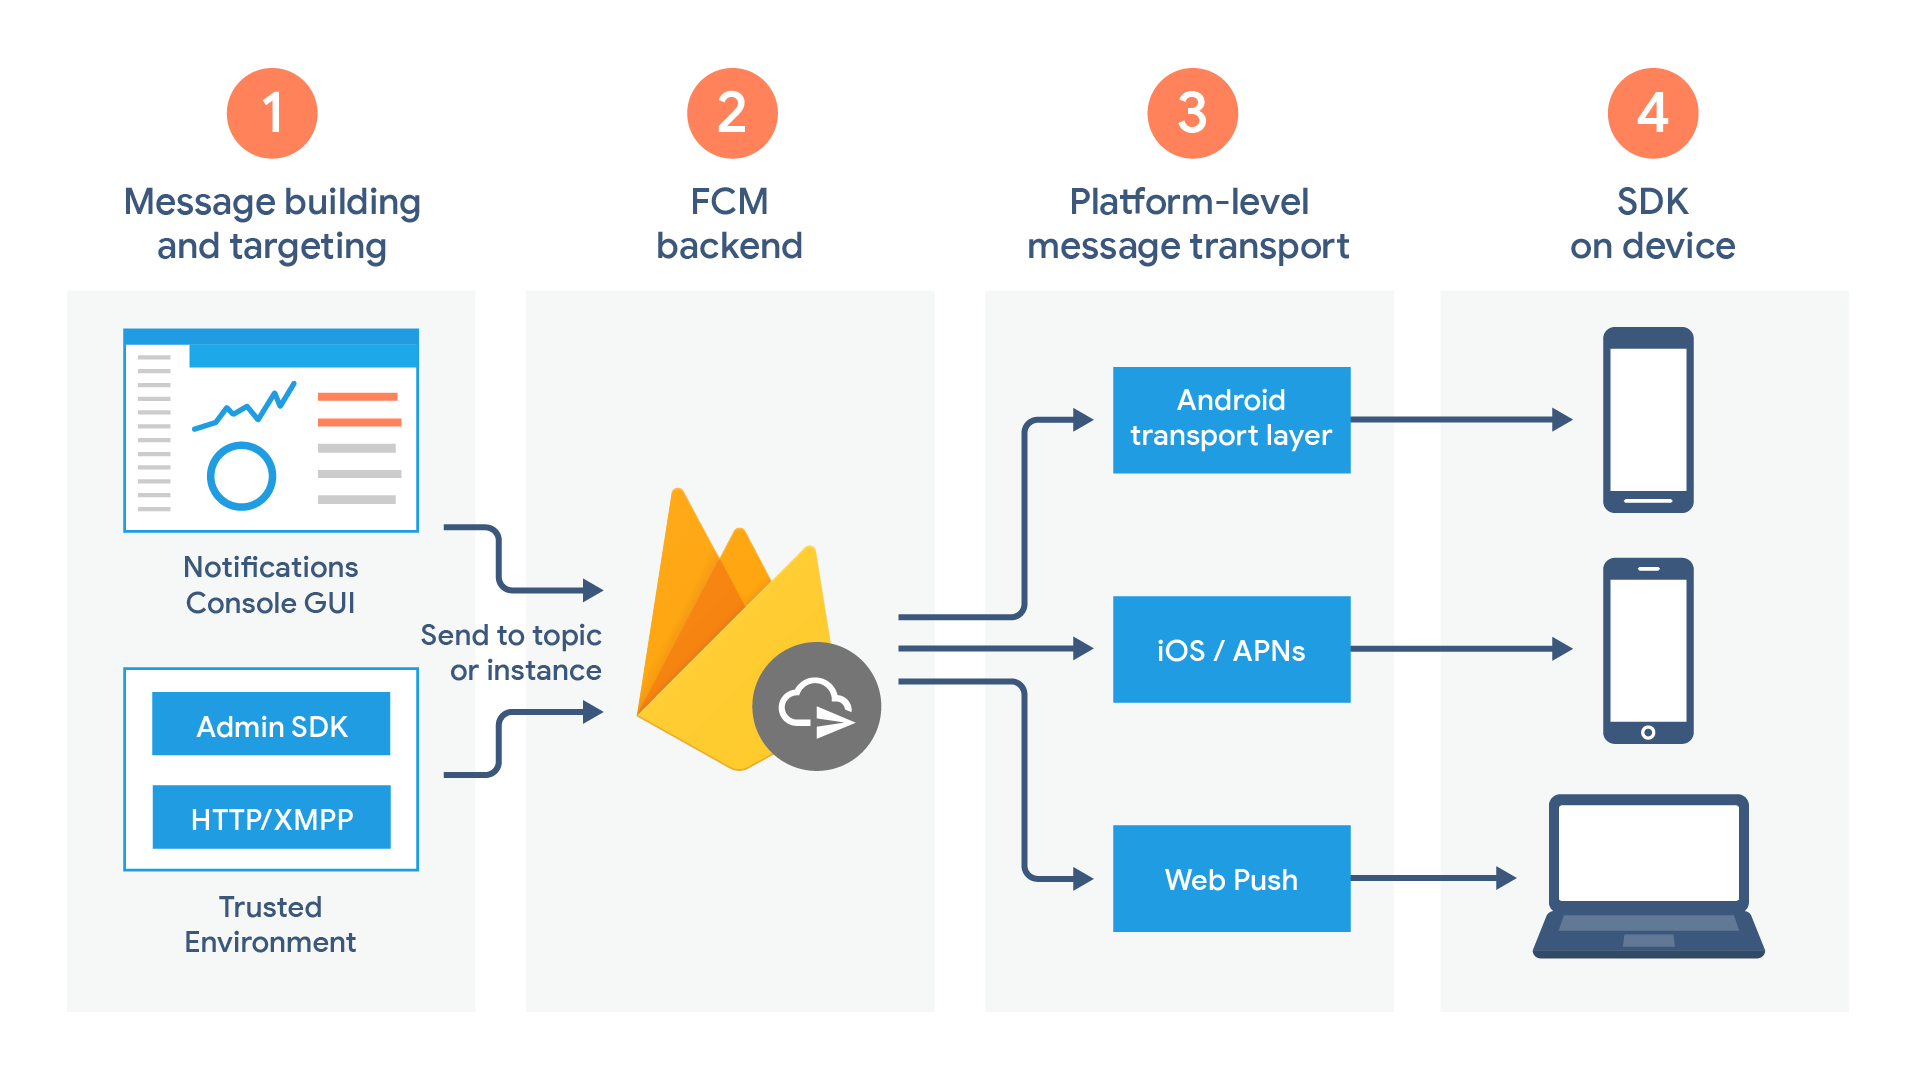
\includegraphics[width=14cm,keepaspectratio]{Images/notifications/diagram-FCM.png}

\noindent Each physical device is registered to a 'topic' which corresponds to the family id and a topic name is essentially an identifier for a pool of observers waiting for possible notifications.
\newline\newline
\noindent To sent notifications programmatically, we made use of \textit{Firebase functions}. We attached three different listeners on new additions on shopping lists, products and users. There is also a scheduled function programmed to run each day at 7a.m. and inform users is a product is expiring that day (Crontab notation).

\vspace*{0.5cm}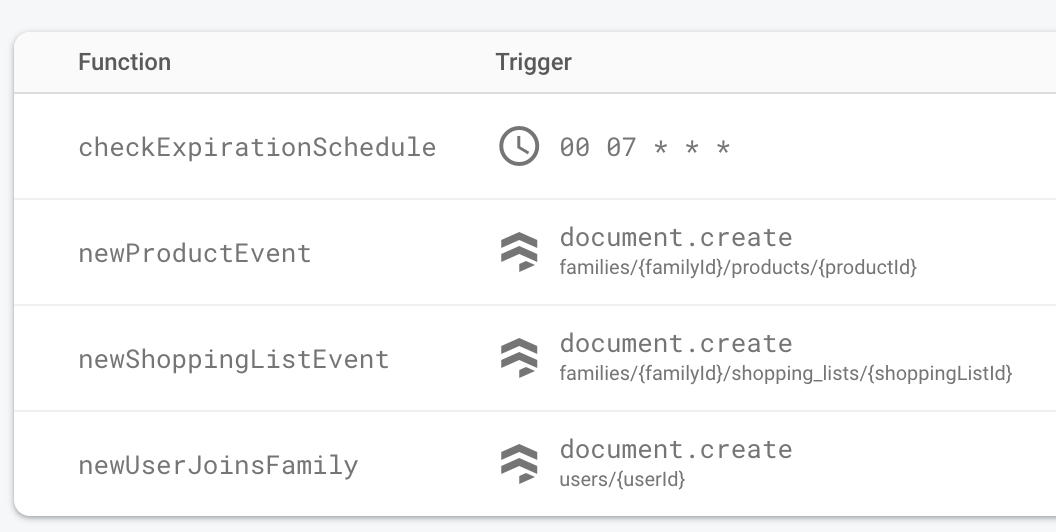
\includegraphics[width=10cm,keepaspectratio]{Images/notifications/firebase_functions.png}

